% =====================================================================
%  CAPÍTULO 4 -- ESTRATÉGIAS DE IMPLEMENTAÇÃO
%  (Regulamento, Art. 9º, item iv; Art. 10 -- protótipo)
% ---------------------------------------------------------------------
%  Fonte: repositório andreccoelho/roundup_app (branch dev), incluindo
%  docs/decisoes-tecnicas.md e docs/DECISOES_PENDENTES.md.
% =====================================================================

\chapter{Estratégias de implementação}
\label{cap:implementacao}

O protótipo do RoundUp é um aplicativo \textbf{codificado e funcional},
e não apenas um protótipo navegável. Antes da codificação, as telas
principais foram desenhadas como \textit{wireframes} de baixa fidelidade
(17 telas) e organizadas no Figma em três páginas: visão do aluno, visão
do gestor (professor e academia) e cadastro inicial, atendendo ao RNF09.
A implementação aconteceu \textbf{em paralelo} à avaliação das ideias,
entre setembro e novembro de 2026, e os resultados do questionário com
usuários reais foram usados para revisar a situação dos requisitos
(\autoref{sec:rf}).

\section{Tecnologias e ferramentas}

O \autoref{qua:tecnologias} apresenta as tecnologias adotadas e a
justificativa de cada escolha.

\begin{quadro}[!htb]
  \caption{Tecnologias e ferramentas}
  \label{qua:tecnologias}
  \centering
  \footnotesize
  \begin{tabular}{|p{3.2cm}|p{4.0cm}|p{6.0cm}|}
    \hline
    \textbf{Finalidade} & \textbf{Tecnologia} & \textbf{Justificativa} \\ \hline
    Aplicativo móvel & React Native com Expo (SDK 58) e TypeScript & Base de código única para Android 7.0+, iOS 16.4+ e web (RNF05); tipagem estática reduz erros entre telas e serviços. \\ \hline
    Navegação & React Navigation & Abas e pilhas de telas separadas por perfil. \\ \hline
    Autenticação & Firebase Authentication & Senhas tratadas pelo provedor, sem armazenamento próprio (RNF03). \\ \hline
    Banco de dados & Cloud Firestore & Banco de documentos gerenciado, com regras de segurança declarativas (RNF04). \\ \hline
    Arquivos & Cloud Storage & Fotos de perfil (RF06), com regras próprias. \\ \hline
    Lógica no servidor & Cloud Functions & Tarefas que o cliente não pode fazer com segurança: listas de leitores, público e progresso de missões, registro de medalhas, exclusão de conta e envio de notificações. \\ \hline
    Notificações & Expo Notifications & Registro do aparelho e envio de notificações \textit{push} (RF31). \\ \hline
    Interface & Expo Blur e Expo System UI & Barras translúcidas e acompanhamento do tema claro ou escuro do aparelho. \\ \hline
    Testes & Jest e Firebase Emulator Suite & Testes unitários e testes das regras de segurança e das funções em emulador local. \\ \hline
    Prototipação & Figma & Validação de telas e fluxos antes da codificação (RNF09). \\ \hline
    Modelagem & PlantUML & Diagramas UML versionáveis como texto. \\ \hline
    Gestão do projeto & Notion e Git/GitHub & Base de requisitos e \textit{backlog}; histórico de alterações por ciclo (RNF08). \\ \hline
    Respostas sintéticas & Claude (\texttt{claude-opus-5-5}), Python e Google Apps Script & Apoio à criação das personas e do gerador de respostas; envio das respostas de teste a uma cópia do formulário (\autoref{sec:val-personas}). \\ \hline
  \end{tabular}
  \fonte{Elaborado pelo autor (2026).}
\end{quadro}

\section{Arquitetura do aplicativo}

O código foi organizado em camadas. As \textbf{telas}
(\texttt{src/screens}), separadas por perfil (aluno, gestor, academia e
telas compartilhadas), cuidam apenas da apresentação e do estado da
interface. Os \textbf{serviços} (\texttt{src/services}), um por coleção do
banco, concentram o acesso ao Firestore e as transações. As
\textbf{regras de gamificação} ficam em funções puras
(\texttt{src/utils/gamificacao.ts}). Os valores ajustáveis, como pontos
por presença e tabela de níveis, podem ser configurados por cada professor
ou academia (RF33); quando não há configuração, valem os valores-padrão
de \texttt{src/config/gamificacao.ts}. As tarefas que dependem de dados de
vários usuários, como manter as listas de leitores, atualizar o público e o
progresso das missões, registrar medalhas, excluir uma conta em cascata e
enviar notificações, ficam em
\textbf{Cloud Functions} (\texttt{functions/src}). O código-fonte
completo, com as regras de segurança, as suítes de testes e a
documentação das decisões técnicas, está no repositório público
\url{https://github.com/andreccoelho/roundup_app}. A segurança não depende do
aplicativo: as \textbf{regras do Firestore} (\texttt{firestore.rules})
validam cada leitura e escrita no servidor, de modo que um cliente
modificado não consegue, por exemplo, creditar pontos a si mesmo.

As telas de professor e de academia compartilham a mesma estrutura de
navegação de ``gestor'' (turmas, alunos e missões), e a academia recebe
abas adicionais para gerenciar professores e consultar a visão
consolidada. Isso reproduz no código a generalização entre os atores
descrita no \autoref{cap:modelagem}.

\section{Etapas de desenvolvimento}

O desenvolvimento seguiu os quatro ciclos definidos nos requisitos, do
núcleo para os recursos complementares:

\begin{enumerate}
  \item \textbf{Ciclo 1 -- base} (início de setembro de 2026): cadastro e
        autenticação dos três perfis, vínculos com solicitação e aceite,
        turmas, matrículas, sessões, \textit{check-in} com janela de tempo,
        agenda e histórico (RF01 a RF08, RF10 a RF15), além das regras de
        segurança e da primeira suíte de testes em emulador;
  \item \textbf{Ciclo 2 -- gamificação}: crédito de XP após validação,
        nível e progresso, medalhas, sequência, missões e classificação
        (RF16 a RF21);
  \item \textbf{Ciclo 3 -- gestão}: validação de presença (chamada),
        criação de missões, lista de alunos com frequência, registro de
        graduação, relatório de frequência, visão consolidada e
        encerramento de vínculos (RF09, RF22 a RF27);
  \item \textbf{Ciclo 4 -- conformidade e retenção} (meados de setembro):
        consentimento LGPD no cadastro, exclusão de conta, responsável
        legal para menores, preferências de notificação e sinalização de
        queda de frequência (RF28 a RF32);
  \item \textbf{Fechamento} (início de novembro): conclusão dos itens
        que tinham ficado parciais, como a exclusão de conta em cascata, a
        classificação mensal com adesão opcional, o progresso das missões,
        a personalização da pontuação, o envio de notificações e a
        sequência contada por sessões. Na reta final, os dados pessoais
        (e-mail, data de nascimento e responsável legal) foram movidos
        para um documento privado do usuário (RNF04), a política de
        privacidade ganhou texto definitivo (RF28), a graduação passou a
        ser registrada por modalidade, escolhida em lista e alterada só
        pelo professor ou pela academia depois do cadastro (RF06, RF25,
        RN03), o gestor passou a alterar o horário e excluir turmas
        (RF10, RF12), e aluno e professor passaram a encerrar vínculos e
        o aluno a sair de turmas (RF07, RF08, RF11);
  \item \textbf{Conclusão dos requisitos parciais} (meados de novembro):
        medalhas persistidas com data de conquista (RF19), público-alvo e
        vigência das missões (RF23), estrutura de faixas personalizável
        por modalidade, com barra de progresso até a próxima graduação
        (RF33 e RF25), e preparação do envio de notificações para teste em
        aparelho (RF31). Nessa etapa, o Expo SDK foi atualizado da versão
        57 para a 58, e a execução do aplicativo em um iPhone revelou
        defeitos que foram corrigidos
        (\autoref{sec:defeitos-testes});
  \item \textbf{Refinamento de interface} (outubro e novembro): três
        rodadas de \textit{redesign}. A última seguiu as diretrizes de
        interface da Apple (\textit{Human Interface Guidelines}), com temas
        claro e escuro que acompanham o aparelho, fonte e escala tipográfica
        do sistema, listas agrupadas, barras translúcidas e anel de
        progresso, preservando a marca, o vermelho de destaque e um fundo
        discreto de lona de ringue nos cartões principais.
\end{enumerate}

A \autoref{fig:telas} mostra seis telas do protótipo na versão final
da interface.

\begin{figure}[!htb]
  \centering
  \caption{Telas do protótipo: (a) acesso; (b) início do aluno; (c) classificação; (d) perfil do aluno; (e) missões; (f) chamada do professor}
  \label{fig:telas}
  \setlength{\fboxsep}{0pt}\setlength{\fboxrule}{0.3pt}
  \begin{tabular}{ccc}
    \fbox{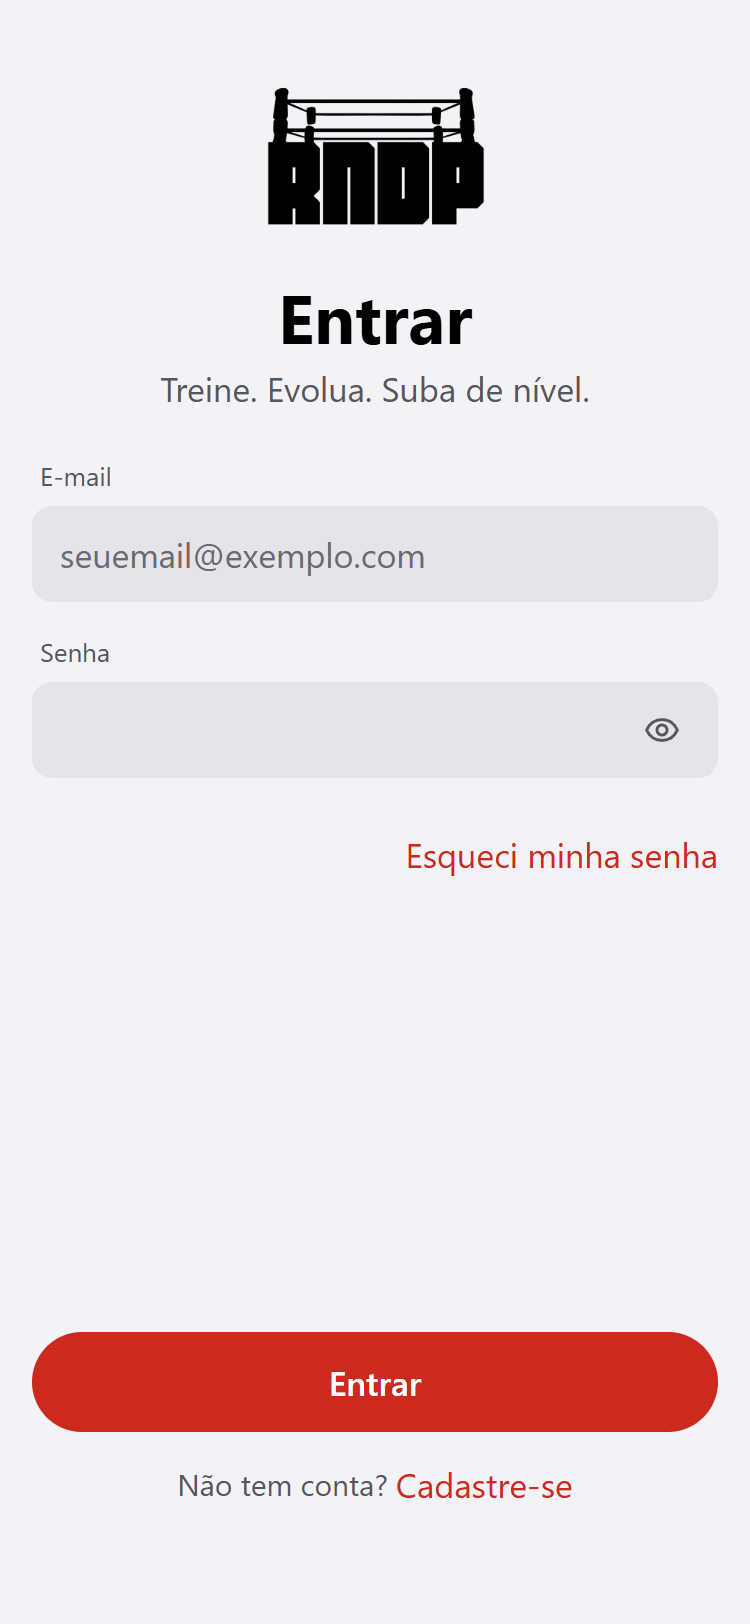
\includegraphics[width=0.27\textwidth]{figuras/tela-login.png}} &
    \fbox{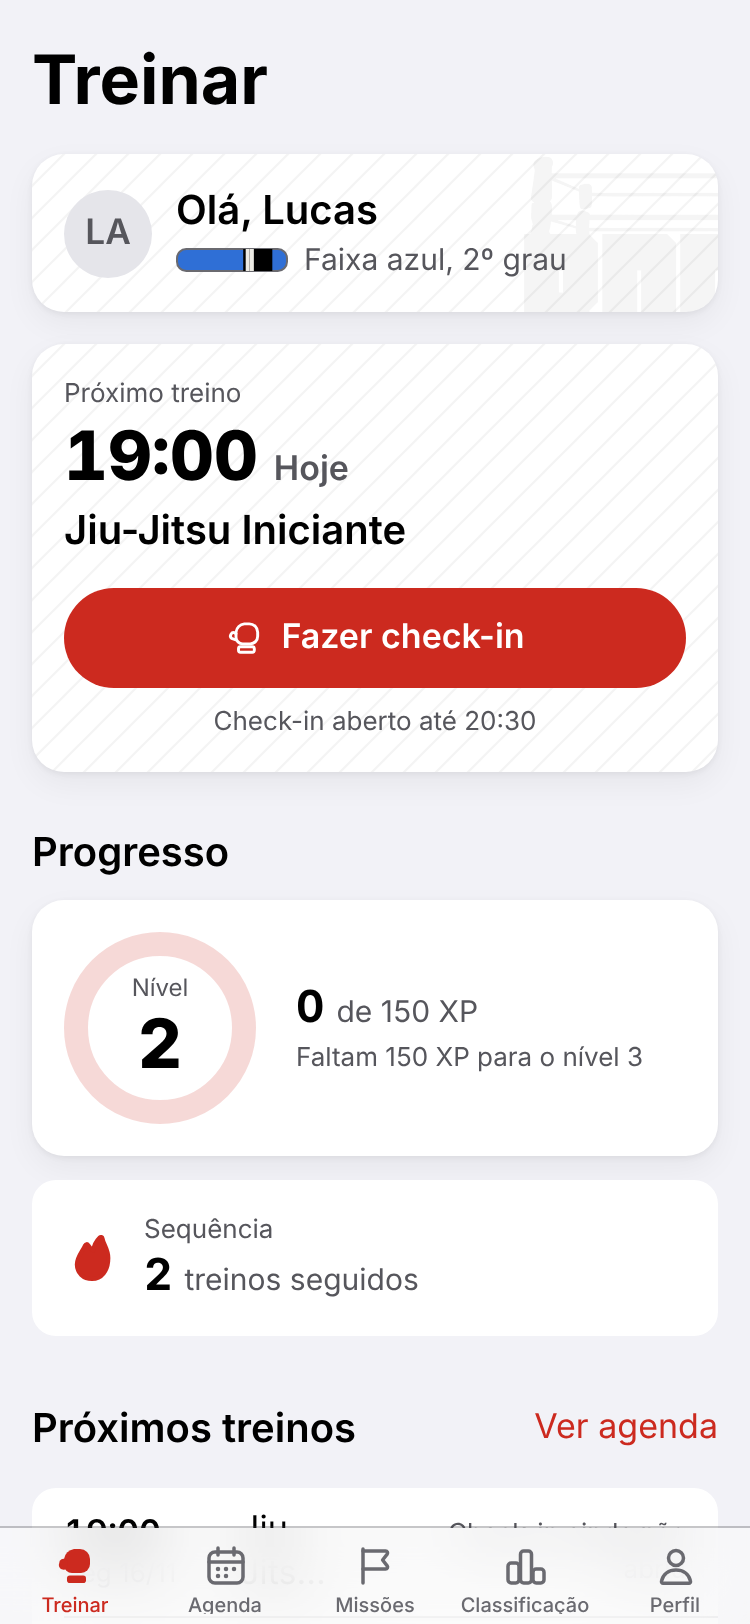
\includegraphics[width=0.27\textwidth]{figuras/tela-aluno-inicio.png}} &
    \fbox{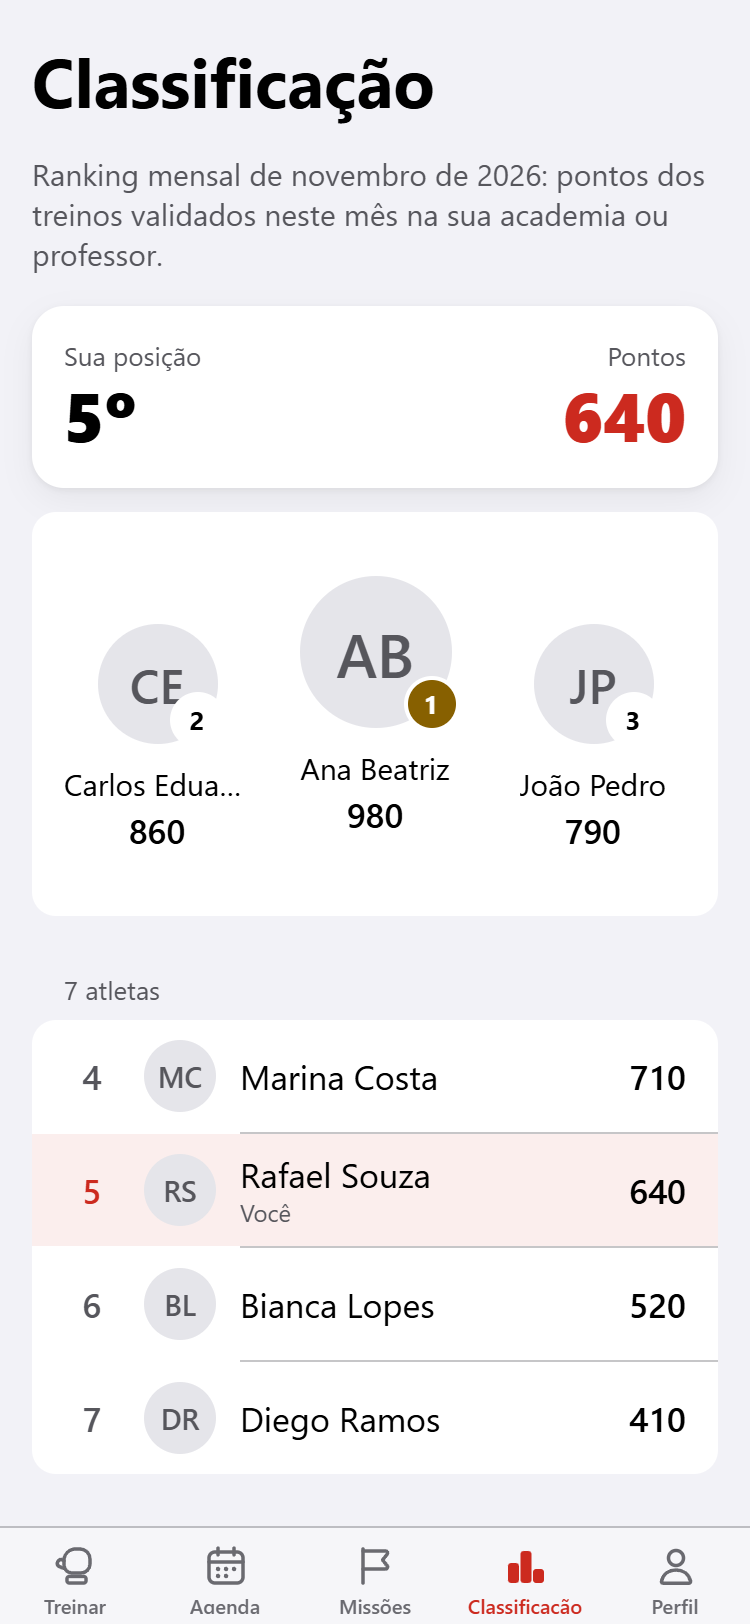
\includegraphics[width=0.27\textwidth]{figuras/tela-aluno-classificacao.png}} \\
    \footnotesize (a) & \footnotesize (b) & \footnotesize (c) \\[6pt]
    \fbox{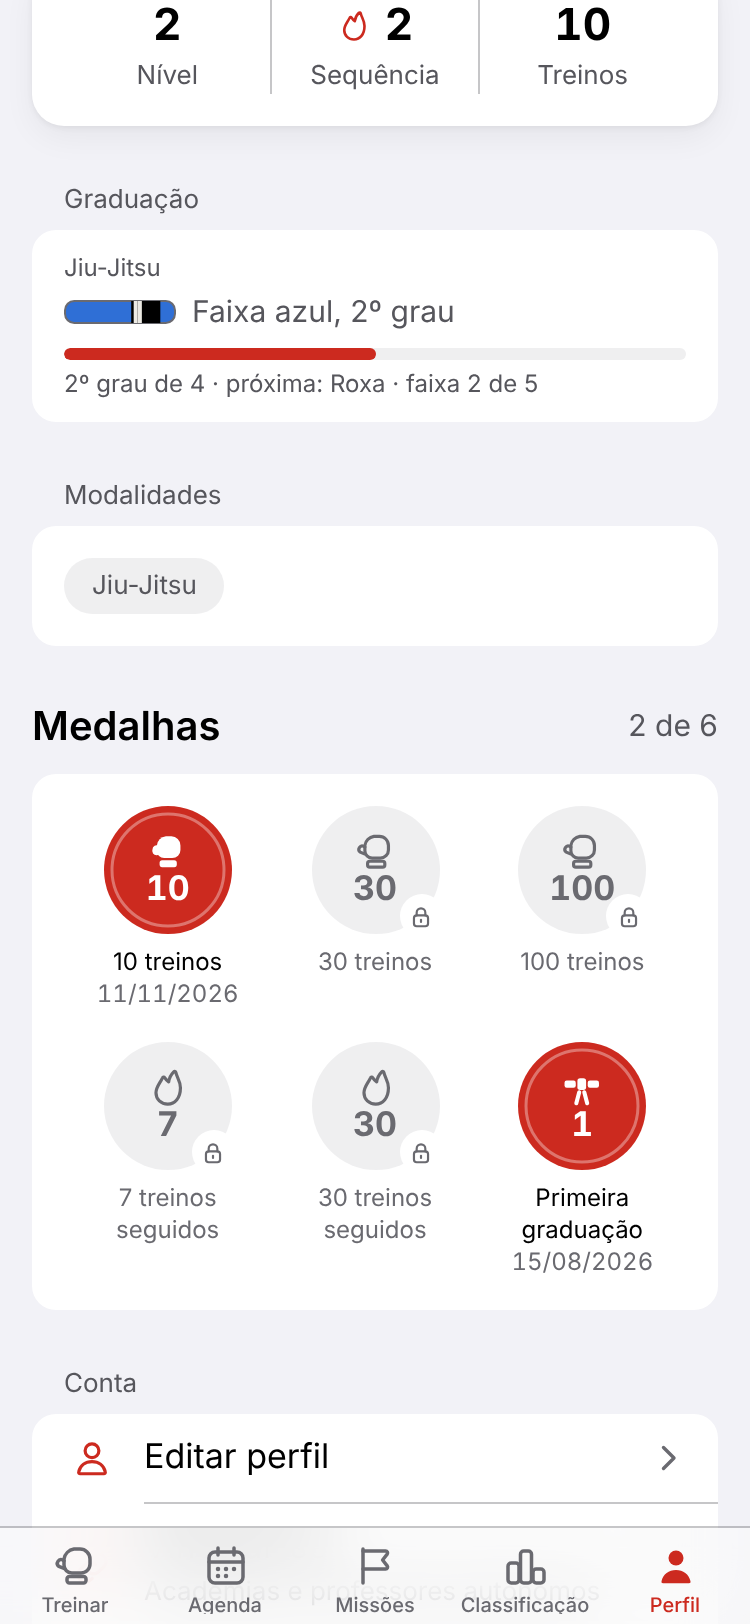
\includegraphics[width=0.27\textwidth]{figuras/tela-aluno-perfil.png}} &
    \fbox{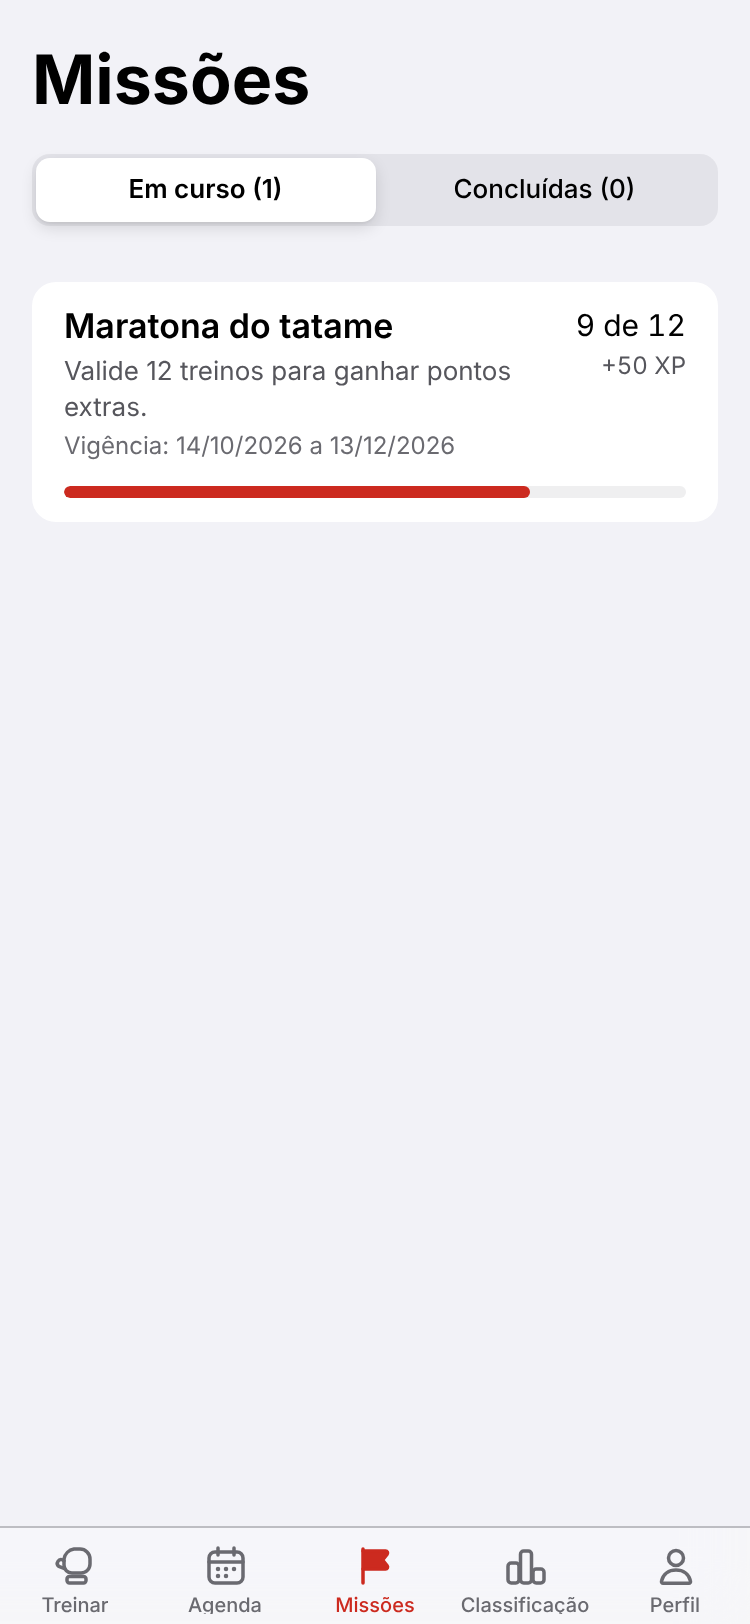
\includegraphics[width=0.27\textwidth]{figuras/tela-aluno-missoes.png}} &
    \fbox{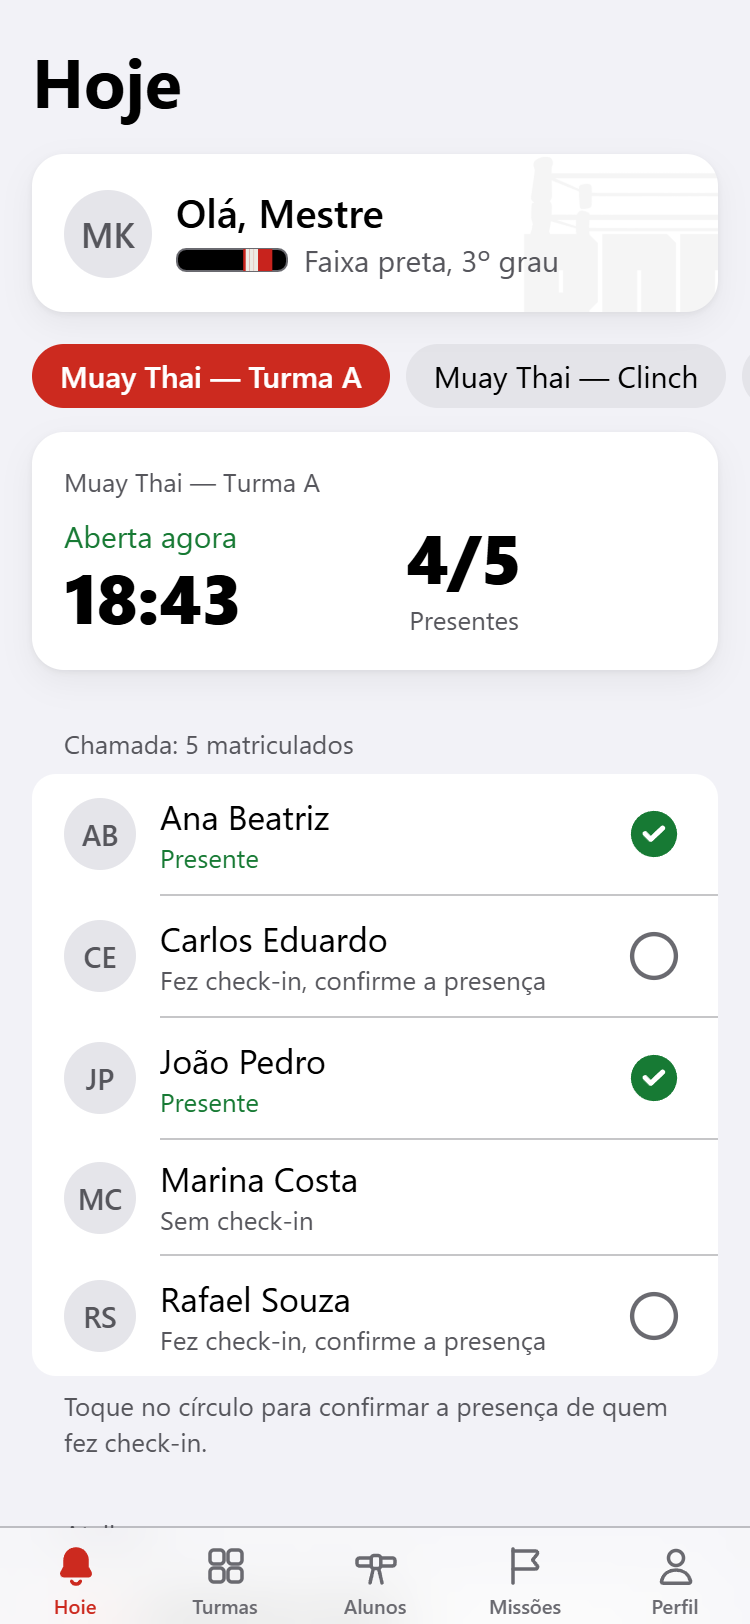
\includegraphics[width=0.27\textwidth]{figuras/tela-professor-chamada.png}} \\
    \footnotesize (d) & \footnotesize (e) & \footnotesize (f)
  \end{tabular}
  \fonte{Elaborado pelo autor (2026). Tema claro; as telas (b) a (f) foram
         capturadas na versão web, com dados fictícios.}
\end{figure}

Na tela inicial do aluno (b), o cartão do próximo treino traz o botão de
\textit{check-in} a um toque de distância, o que atende ao RNF01; logo
abaixo aparecem o anel de progresso, com o nível e o XP que falta para o
próximo, e a sequência de treinos. Na classificação (c), o aluno vê a sua
posição no mês e a linha dele aparece destacada. No perfil (d), a barra
de graduação mostra o grau atual dentro da faixa e a próxima faixa da
estrutura do responsável (RF33), e as medalhas conquistadas exibem a data
da conquista (RF19). Nas missões (e), cada missão mostra o progresso, a
recompensa e o período de vigência (RF23). Na chamada do professor (f),
cada aluno que fez \textit{check-in} tem a presença confirmada com um
toque no círculo.

\section{Situação de implementação dos requisitos}
\label{sec:situacao-implementacao}

O \autoref{qua:implementacao} resume o que foi implementado. As
limitações remanescentes foram registradas no repositório como decisões
pendentes, para que fiquem explícitas, e não escondidas na interface. O
critério de compatibilidade do RNF05 foi revisado de iOS 14 para iOS
16.4, versão mínima exigida pelo Expo SDK 58, adotado na etapa final; no
Android, o mínimo do SDK (Android 7.0) já atende ao critério original.

\begin{quadro}[!htb]
  \caption{Situação de implementação dos requisitos}
  \label{qua:implementacao}
  \centering
  \footnotesize
  \begin{tabular}{|p{2.2cm}|p{4.2cm}|p{7.0cm}|}
    \hline
    \textbf{Situação} & \textbf{Requisitos} & \textbf{Observação} \\ \hline
            Implementado & RF01--RF33; RN01--RN09; RNF01--RNF05, RNF07--RNF11 & Funcionalidades disponíveis nas telas e cobertas, na parte de segurança e de servidor, por testes em emulador. RF19, RF23, RF31 e RF33 também foram verificados em um iPhone, e o tempo de carregamento (RNF02) foi medido em 4G (\autoref{sec:testes-prototipo}). \\ \hline
    Não implementado & RNF06 & Decisão de projeto: o \textit{check-in} e a validação de presença são gravados em transações que exigem conexão, porque o servidor precisa garantir a janela de horário (RN08) e o limite de um \textit{check-in} por sessão (RN02). Um registro feito sem conexão poderia ser recusado depois, quando o aluno já acreditasse ter treinado com pontos garantidos. \\ \hline
  \end{tabular}
  \fonte{Elaborado pelo autor (2026), a partir do repositório do projeto.}
\end{quadro}

Os valores de gamificação têm um padrão, usado quando o professor ou a
academia não configuram os seus: 10 pontos por presença validada, dez
níveis com limiares crescentes (100, 250, 450\ldots{} até 3.250 pontos) e
medalhas para 10, 30 e 100 treinos, para sequências de 7 e 30 sessões e
para a primeira graduação. Esses valores permitiram construir e testar a
interface, mas ainda precisam ser calibrados com uso real.

Na conclusão dos requisitos que estavam parciais, quatro decisões
merecem registro:

\begin{itemize}
  \item \textbf{Medalhas (RF19).} Cada medalha é gravada em
        \texttt{usuarios/\{aluno\}/medalhas}, com a data de conquista,
        somente por Cloud Function; o aplicativo não consegue escrevê-la.
        O estorno de um \textit{check-in} não retira uma medalha já
        conquistada, e um \textit{script} de migração reconstruiu, a partir
        do histórico, a data das medalhas dos alunos existentes.
  \item \textbf{Missões (RF23).} O gestor define o público (todos os alunos
        vinculados, uma turma ou alunos escolhidos) e a vigência. A regra
        vale no banco de dados, não só na tela: só o público lê a missão,
        a conclusão manual só é aceita dentro da vigência, o progresso
        automático só conta treinos do período e o aviso de nova missão
        (RF31) vai só para o público, uma vez por aluno. Depois do fim da
        vigência, a missão continua no histórico de quem a concluiu.
  \item \textbf{Faixas (RF33).} O gestor personaliza, por modalidade, a
        ordem, o nome, a cor e o número de graus de cada faixa; sem
        personalização, vale a lista anterior como padrão. O registro de
        graduação (RF25) passou a gravar a faixa de forma estruturada, e o
        perfil do aluno ganhou a barra de progresso até a próxima
        graduação, medida pelos graus da faixa atual (por exemplo, ``2º
        grau de 4 · próxima: Roxa''). Graduações antigas, registradas como
        texto livre, foram convertidas por um \textit{script} que reconhece
        o nome da faixa; os textos sem correspondência permanecem como
        texto.
  \item \textbf{Notificações (RF31).} O projeto foi preparado para gerar
        versões instaláveis pelo EAS, e a tela de preferências de
        notificação ganhou botões para enviar uma notificação de teste ao
        próprio aparelho, o que permitiu validar o envio em um iPhone.
\end{itemize}

\section{Detalhes de implementação}

\subsection{Crédito de pontos com validação humana}

O \autoref{cod:validar} mostra o núcleo da função que confirma uma
presença. A confirmação e o crédito acontecem em uma única transação: o
\textit{check-in} recebe os pontos configurados pelo responsável e a
classificação do aluno, no escopo daquele responsável e no mês da sessão,
é atualizada. Se o professor desfizer a confirmação, os pontos são
estornados. A regra de segurança confere o \textit{check-in} e a
classificação na mesma transação: o crédito só pode ser o valor
configurado, e o estorno só pode devolver o que o \textit{check-in}
recebeu. Isso impede créditos arbitrários mesmo que alguém altere o
aplicativo.

\begin{codigo}[!htb]
  \caption{Validação de presença e crédito de pontos (TypeScript, trecho)}
  \label{cod:validar}
\begin{lstlisting}
await runTransaction(db, async (transacao) => {
  const checkin = (await transacao.get(checkinRef)).data() as CheckIn;
  const vaiCreditar = novoStatus === 'validado' && checkin.pontos === 0;
  const vaiEstornar = novoStatus === 'pendente' && checkin.pontos > 0;
  const periodo = periodoDe(checkin.dataHora.toDate());          // AAAA-MM
  const classificacaoId = vaiEstornar && checkin.classificacaoId
    ? checkin.classificacaoId
    : `${checkin.alunoId}_${checkin.responsavelId}_${periodo}`;
  const classificacaoRef = doc(db, 'classificacoes', classificacaoId);
  let pontosAtuais = 0, pontosDoCheckin = 0;
  if (vaiCreditar || vaiEstornar) {
    const snap = await transacao.get(classificacaoRef);
    pontosAtuais = snap.exists() ? snap.data().pontos : 0;
  }
  if (vaiCreditar) {                    // valor configurado ou padrao (RF33)
    const config = await transacao.get(doc(db, 'configuracoesGamificacao',
                                           checkin.responsavelId));
    pontosDoCheckin = config.exists() ? config.data().pontosPorCheckin
                                      : XP_POR_CHECKIN_VALIDADO;
  }
  transacao.update(checkinRef, {
    status: novoStatus, validadoPor: responsavelId,
    pontos: vaiCreditar ? pontosDoCheckin : vaiEstornar ? 0 : checkin.pontos,
    ...(vaiCreditar || vaiEstornar ? { classificacaoId } : {}),
  });
  if (vaiCreditar || vaiEstornar) {
    const delta = vaiCreditar ? pontosDoCheckin : -checkin.pontos;
    transacao.set(classificacaoRef, { pontos: pontosAtuais + delta,
      periodo: classificacaoId.slice(-7), origemCheckinId: checkinId },
      { merge: true });
  }
});
\end{lstlisting}

  \fonte{Elaborado pelo autor (2026), adaptado de \texttt{src/services/checkins.ts}.}
\end{codigo}

\subsection{Cálculo da sequência de treinos}

A sequência (RF21) conta as \textbf{sessões consecutivas} das turmas do
aluno em que ele teve presença validada, da mais recente para a mais
antiga (\autoref{cod:sequencia}). Sessões canceladas não contam, e uma
sessão com a janela de \textit{check-in} ainda aberta, ou com
\textit{check-in} aguardando validação, é ignorada, para não interromper a
sequência antes da hora. Assim, um dia sem aula não quebra a sequência:
ela só é interrompida quando houve sessão e o aluno não compareceu. O
mesmo critério é usado no aplicativo e nas Cloud Functions que avaliam as
missões de sequência.

\begin{codigo}[!htb]
  \caption{Cálculo da sequência de treinos por sessão (TypeScript)}
  \label{cod:sequencia}
\begin{lstlisting}
export function calcularSequencia(sessoes: Sessao[], checkins: CheckIn[],
                                  agora: Date = new Date()): number {
  const statusPorSessao = new Map(checkins.map((c) => [c.sessaoId, c.status]));
  const maisRecentesPrimeiro = sessoes
    .filter((s) => s.status !== 'cancelada')
    .sort((a, b) => b.janelaCheckInFim.toMillis() - a.janelaCheckInFim.toMillis());
  let sequencia = 0;
  for (const sessao of maisRecentesPrimeiro) {
    const status = statusPorSessao.get(sessao.id);
    if (status === 'validado') sequencia += 1;
    else if (sessao.janelaCheckInFim.toDate() > agora || status === 'pendente') continue;
    else break;                         // houve sessao e o aluno nao foi
  }
  return sequencia;
}
\end{lstlisting}
  \fonte{Elaborado pelo autor (2026), adaptado de \texttt{src/utils/gamificacao.ts}.}
\end{codigo}

